\documentclass[nobib]{tufte-handout}

\usepackage{amssymb}
\usepackage{hyperref}
\usepackage{pgfplots}
\usepackage[activate={true,nocompatibility},final,tracking=true,kerning=true,spacing=true,factor=1100,stretch=10,shrink=10]{microtype}
\usepackage{color}
\usepackage{steinmetz}
\usepackage{placeins}
\usepackage{marginfix}
\usepackage{array}
\usepackage{tikz}
\usepackage{amsmath}
\usepackage{amsthm}
\usepackage{booktabs}
\usepackage{listings}
\usepackage[edges]{forest}
\usepackage{caption}
\usepackage[T1]{fontenc}
\usepackage{lmodern}
\usepackage{units}
\usepackage{fancyvrb}
\usepackage{multicol}
\DeclareCaptionFont{white}{\color{white}}
\DeclareCaptionFormat{listing}{\colorbox{gray}{\parbox{\textwidth}{#1#2#3}}}
\captionsetup[lstlisting]{format=listing,labelfont=white,textfont=white}

% Set up the images/graphics package
\usepackage{graphicx}
\setkeys{Gin}{width=\linewidth,totalheight=\textheight,keepaspectratio}
\graphicspath{{.}}

\title{Notes for ECE 30834 - Fundamentals of Computer Graphics}
\author{Zeke Ulrich}
\date{\today} 

\fvset{fontsize=\normalsize}
\usetikzlibrary{shapes}
\usetikzlibrary{positioning}

% For finite state machines 
\usetikzlibrary{automata} % Import library for drawing automata
\usetikzlibrary{positioning} % ...positioning nodes
\usetikzlibrary{arrows} % ...customizing arrows
\tikzset{node distance=2.5cm, % Minimum distance between two nodes. Change if necessary.
    every state/.style={ % Sets the properties for each state
    semithick,
    fill=gray!10},
    initial text={}, % No label on start arrow
    double distance=2pt, % Adjust appearance of accept states
    every edge/.style={ % Sets the properties for each transition
    draw,
    ->,>=stealth', % Makes edges directed with bold arrowheads
    auto,
    semithick}}
\let\epsilon\varepsilon

% These commands are used to pretty-print LaTeX commands
\newcommand{\doccmd}[1]{\texttt{\textbackslash#1}}% command name -- adds backslash automatically
\newcommand{\docopt}[1]{\ensuremath{\langle}\textrm{\textit{#1}}\ensuremath{\rangle}}% optional command argument
\newcommand{\docarg}[1]{\textrm{\textit{#1}}}% (required) command argument
\newenvironment{docspec}{\begin{quote}\noindent}{\end{quote}}% command specification environment
\newcommand{\docenv}[1]{\textsf{#1}}% environment name
\newcommand{\docpkg}[1]{\texttt{#1}}% package name
\newcommand{\doccls}[1]{\texttt{#1}}% document class name
\newcommand{\docclsopt}[1]{\texttt{#1}}% document class option name

% Define a custom command for definitions and biconditional
\newcommand{\defn}[2]{\noindent\textbf{#1}:\ #2}
\let\biconditional\leftrightarrow

\begin{document}

\maketitle

\tableofcontents

\section{Course Description}
Fundamental principles and techniques of computer graphics. The course covers the basics of going from a scene representation to a raster image using OpenGL. Specific topics include coordinate manipulations, perspective, basics of illumination and shading, color models, texture maps, clipping and basic raster algorithms, fundamentals of scene constructions.
\pagebreak

\section{Introduction}
Let's examine some basic C++ programs.
\begin{lstlisting}[language=C++,caption=Hello World]
    #include <iostream>

    int main() {
        std::cout << "Hello World!";
        return 0;
    }
\end{lstlisting}

\begin{lstlisting}[language=C++,caption=User Input]
    #include <iostream>

    int main() {
        double n;
        int i;

        std::cout << "Enter float: ";
        std::cin >> n;

        std::cout << "Enter integer: ";
        std::cin >> i;

        return 0;
    }
\end{lstlisting}

The \texttt{stds} you're seeing all over the place refer not
to a frat party but the standard namespace. It holds
useful objects like standard in ("\texttt{cin}") and standard
out ("\texttt{cout}").

In C, we use \texttt{malloc} and \texttt{free} to allocate memory. In C++,
the equivalent operations are \texttt{new} and \texttt{delete}.

\begin{lstlisting}[language=C++,caption=Free and Delete]
    void CorrectUsage(){
        int *ptr = new int[3];
        int *ptr1 = new int;
        ptr[0] = 1;
        ptr[1] = 2;
        ptr[2] = 3;
        *ptr1 = 5;
        delete ptr1;
        delete [] ptr;        
\end{lstlisting}
The reason for this is using \texttt{new} and \texttt{free} calls
an object's constructor and destructors, which are defined to properly
delete the object. Technically, \texttt{malloc} and \texttt{free} are
both present in C++, but they won't trigger the constructors and
destructors and should be avoided. The choice to leave these functions in
was made to improve compatibility with C, which is a theme the reader
may notice in C++'s many possible ways to do the same thing.

C++ filenames are terminated with a \texttt{.cpp} or \texttt{.cc}
extension, like \texttt{example.cpp} or \texttt{example.cc}
\section{Linear Algebra}

\subsection{Points and Vectors}
In three-dimensional space like ours, we require three numbers to
specify a point. These numbers only make sense with reference to
a coordinate system, typically an origin and set of axes like with
Cartesian coordinates.

\begin{equation}\mathbf{p} = \begin{pmatrix} x \\ y \\ z \end{pmatrix}\end{equation}
\begin{equation}d(P_1, P_2) = \sqrt{(x_2 - x_1)^2 + (y_2 - y_1)^2 + (z_2 - z_1)^2}\end{equation}
\begin{equation}\mathbf{v} = \begin{pmatrix} v_x \\ v_y \\ v_z \end{pmatrix} = (v_x, v_y, v_z)\end{equation}
\begin{equation}|\mathbf{v}| = \sqrt{v_x^2 + v_y^2 + v_z^2}\end{equation}
\begin{equation}\hat{\mathbf{v}} = \frac{\mathbf{v}}{|\mathbf{v}|} = \frac{1}{\sqrt{v_x^2 + v_y^2 + v_z^2}}\begin{pmatrix} v_x \\ v_y \\ v_z \end{pmatrix}\end{equation}

\subsection{Directions}
A direction goes from one point to another, but its location
in space doesn't matter. A direction starting at the origin
going straight up is the same as a direction starting anywhere
else going straight up. Its length doesn't matter either, so
we generally keep it as length 1. We represent directions
with 3D vectors, like $(1, 2, 3)$.

\subsection{Dot Product}
The dot product takes in two vectors and produces a number.
\begin{equation}\mathbf{a} \cdot \mathbf{b} = a_x b_x + a_y b_y + a_z b_z = |\mathbf{a}||\mathbf{b}|\cos\theta\end{equation}
where $\theta$ is the angle between the vectors.

\subsection{Cross Product}
The cross product takes two vectors and returns a vector.
\begin{equation}\mathbf{a} \times \mathbf{b} = \begin{pmatrix} a_y b_z - a_z b_y \\ a_z b_x - a_x b_z \\ a_x b_y - a_y b_x \end{pmatrix}\end{equation}

\subsection{Matrix-vector Multiplication}
Vectors and matrices can be multiplied.
\begin{equation}\begin{pmatrix} m_{11} & m_{12} & m_{13} \\ m_{21} & m_{22} & m_{23} \\ m_{31} & m_{32} & m_{33} \end{pmatrix} \begin{pmatrix} v_x \\ v_y \\ v_z \end{pmatrix} = \begin{pmatrix} m_{11}v_x + m_{12}v_y + m_{13}v_z \\ m_{21}v_x + m_{22}v_y + m_{23}v_z \\ m_{31}v_x + m_{32}v_y + m_{33}v_z \end{pmatrix}\end{equation}

\subsection{Planes}

A plane in three-dimensional space can be defined in several equivalent ways. One common form uses a point on the plane and a normal vector $\mathbf{n} = (a, b, c)$ perpendicular to the plane.

\begin{equation}
    a(x - x_0) + b(y - y_0) + c(z - z_0) = 0
\end{equation}

This is the point-normal form of the plane, where $(x_0, y_0, z_0)$ is a known point on the plane. It can also be written as:

\begin{equation}
    ax + by + cz = d
\end{equation}
where $d = ax_0 + by_0 + cz_0$.

If three non-collinear points $P_1$, $P_2$, and $P_3$ lie on a plane, we can compute two vectors from them:

\begin{equation}
    \mathbf{v}_1 = \overrightarrow{P_1P_2}, \quad \mathbf{v}_2 = \overrightarrow{P_1P_3}
\end{equation}

Then, the cross product of these vectors gives a normal vector to the plane:

\begin{equation}
    \mathbf{n} = \mathbf{v}_1 \times \mathbf{v}_2
\end{equation}

With this normal and any of the three points, we can construct the plane equation.

\subsection{Triangles}

A triangle in 3D space is defined by three points: $A$, $B$, and $C$. These points form the triangle's vertices. The triangle can be described in terms of its edges, which are vectors:

\begin{equation}
    \mathbf{AB} = \mathbf{B} - \mathbf{A}, \quad \mathbf{AC} = \mathbf{C} - \mathbf{A}, \quad \mathbf{BC} = \mathbf{C} - \mathbf{B}
\end{equation}

The normal of the triangle's plane can be found by:

\begin{equation}
    \mathbf{n} = \mathbf{AB} \times \mathbf{AC}
\end{equation}

This normal is perpendicular to the surface of the triangle and is often used in graphics and geometry processing for lighting and orientation.

The area of the triangle is given by:

\begin{equation}
    \text{Area} = \frac{1}{2} |\mathbf{AB} \times \mathbf{AC}|
\end{equation}

You can also interpolate points inside the triangle using barycentric coordinates, which express any point $P$ in the triangle as a weighted sum of the vertices:

\begin{equation}
    P = \alpha A + \beta B + \gamma C, \quad \text{where } \alpha + \beta + \gamma = 1 \text{ and } \alpha, \beta, \gamma \ge 0
\end{equation}

\subsection{Transformation}

A transformation moves or reorients points, vectors, or shapes in space. The most common transformations are:

\begin{itemize}
    \item Translation: Shifts a point by a vector.
    \item Scaling: Changes the size of an object.
    \item Rotation: Rotates an object around an axis.
    \item Reflection: Flips an object over a plane.
    \item Projection: Projects a point onto a plane or line.
    \item Translating Points and Vectors
\end{itemize}

To translate a point $\mathbf{p}$ by a vector $\mathbf{v}$:

\begin{equation}
    \mathbf{p}' = \mathbf{p} + \mathbf{v}
\end{equation}

Vectors are not affected by translation—they describe direction and magnitude, not position.

To translate a triangle, add the translation vector $\mathbf{t}$ to each vertex:

\begin{equation}
    A' = A + \mathbf{t}, \quad B' = B + \mathbf{t}, \quad C' = C + \mathbf{t}
\end{equation}

The shape and size of the triangle remain unchanged.

Linear transformations like rotation, scaling, and shearing are usually done via matrix-vector multiplication. A 3x3 matrix transforms vectors or points (relative to the origin):

\begin{equation}
    \mathbf{v}' = M\mathbf{v}
\end{equation}

To include translation with linear transformations, we use homogeneous coordinates and 4x4 matrices, which is common in computer graphics.

\subsection{Rotations}

Rotations can be encoded with matrices. In three-dimensional space, rotation is a linear transformation that turns vectors around an axis while preserving their lengths and angles between them.

Given an angle $\theta$, rotating a vector by $\theta$ is accomplished with a rotation matrix. The exact form of the matrix depends on the axis of rotation.

\begin{equation}
    R_x(\theta) =
    \begin{pmatrix}
        1 & 0          & 0           \\
        0 & \cos\theta & -\sin\theta \\
        0 & \sin\theta & \cos\theta
    \end{pmatrix}
\end{equation}
\begin{equation}
    R_y(\theta) =
    \begin{pmatrix}
        \cos\theta  & 0 & \sin\theta \\
        0           & 1 & 0          \\
        -\sin\theta & 0 & \cos\theta
    \end{pmatrix}
\end{equation}
\begin{equation}
    R_z(\theta) =
    \begin{pmatrix}
        \cos\theta & -\sin\theta & 0 \\
        \sin\theta & \cos\theta  & 0 \\
        0          & 0           & 1
    \end{pmatrix}
\end{equation}

To rotate a vector $\mathbf{v}$ about an axis, we multiply it by the corresponding rotation matrix:

\begin{equation}
    \mathbf{v}' = R \mathbf{v}
\end{equation}

For example, rotating $\mathbf{v}$ about the $z$-axis by $\theta$ radians:

\begin{equation}
    \mathbf{v}' = R_z(\theta) \mathbf{v}
\end{equation}

To rotate around an arbitrary unit axis vector $\hat{\mathbf{u}} = (u_x, u_y, u_z)$ by an angle $\theta$, we can use Rodrigues' rotation formula or construct a 3x3 matrix:

\begin{equation}
    R(\hat{\mathbf{u}}, \theta) =
    \cos\theta , I +
    (1 - \cos\theta) , \hat{\mathbf{u}} \hat{\mathbf{u}}^\top +
    \sin\theta , [\hat{\mathbf{u}}]_\times
\end{equation}

Where $I$ is the identity matrix, $\hat{\mathbf{u}} \hat{\mathbf{u}}^\top$
is the outer product, and $[\hat{\mathbf{u}}]_\times$ is the skew-symmetric matrix.

\begin{equation}
    [\hat{\mathbf{u}}]_\times =
    \begin{pmatrix}
        0    & -u_z & u_y  \\
        u_z  & 0    & -u_x \\
        -u_y & u_x  & 0
    \end{pmatrix}
\end{equation}

This general rotation formula allows rotation around any axis, not just the coordinate axes.

\subsection{Changing Coordinate Systems}

Given a point $P$, a new coordinate system defined by an origin $O'$ and
basis vectors $\vec{x}, \vec{y}, \vec{z}$, how do we find the coordinates
of $P$ in this new system?

First, we express the vector from the new origin to  $P$:

\begin{equation}
    \mathbf{v} = \mathbf{P} - \mathbf{O'}
\end{equation}

This gives the position of $P$ relative to the new origin.

Next, we project $\mathbf{v}$ onto the new basis vectors. Assuming the new basis
is orthonormal (i.e. all vectors are unit length and perpendicular to each other),
we compute:

\begin{equation}
    P'_x = \mathbf{v} \cdot \mathbf{x'} \quad
    P'_y = \mathbf{v} \cdot \mathbf{y'} \quad
    P'_z = \mathbf{v} \cdot \mathbf{z'}
\end{equation}

So $P$ in the new coordinate system is:

\begin{equation}
    \mathbf{P'} = \begin{pmatrix} P'_x \\ P'_y \\ P'_z \end{pmatrix}
\end{equation}

Matrix Form (Basis Change Matrix)

You can also express this operation as a matrix multiplication. Let
$R$ be the rotation matrix whose columns are the new basis vectors:

\begin{equation}
    R = \begin{pmatrix}
        |           & |           & |           \\
        \mathbf{x'} & \mathbf{y'} & \mathbf{z'} \\
        |           & |           & |
    \end{pmatrix}
\end{equation}

Then the change of basis is:

\begin{equation}
    \mathbf{P'} = R^\top (\mathbf{P} - \mathbf{O'})
\end{equation}
\section{Cameras}

In graphics, a camera projects a 3D scene onto a 2D plane which
can be displayed on a screen. If we model the camera as a point,
then the problem becomes a linear algebra issue of projecting a
set of points onto a plane determined by the camera. We must
display only surfaces not obscured by other surfaces, not accounting
for things like transparency.

\begin{figure}
    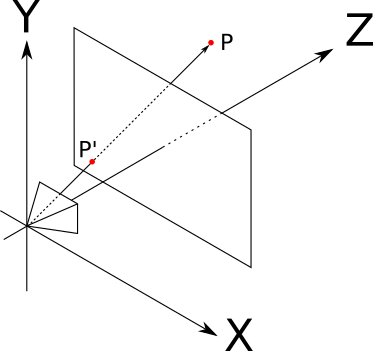
\includegraphics{images/camera.png}
    \caption{Camera}
    \label{fig:camera}
\end{figure}

A \emph{pose} consists of three translations and three rotations.
Setting each results in a unique camera pose in 3D space.

\marginnote{There are several ways to approximate the way the human
    eye sees, the method used in this class is called the planar pinhole method.
    There are many, many other camera models, for instance thin lens camera,
    orthographic camera, spherical camera, fisheye camera.}
\section{Drawing}

Drawing more complex shapes just requires connecting
vectors together and displaying them on screen. We can
translate them, rotate vectors, and shift the camera.

\subsection{Triangles}

In computer graphics, everything is made of triangles.
A \emph{shared-vertex triangle mesh} is a bunch of triangles
who can have the same vertices that forms some shape. A
triangle is fully specified with a triple of unsigned ints
that specify which indices in the array of vertices belong
to that triangle. For instance, with a cube made of 8 vectors,
each triangle needs only specify which three of the vectors
that form the vertices it has.

Once we have the ability to draw triangles, it would be
useful to be able to draw points and wire frames.

\end{document}